\chapter{Software Design}
\section{RTOS Communication Protocol}

Ideally FreeRTOS tasks should operate with as much isolation as possible, with each task performing a specific function with different priority levels. In the case of a communication protocol, the overall task is inherently sequential so this leads to FreeRTOS being used in a sequential way with all tasks operating at real-time priority level. 

FreeRTOS was chosen because of the following benefits:

\begin{enumerate}
\item Segmentation of code into specific tasks provides readable code for future users.
\item FreeRTOS task configuration provides a framework for future embedded robotic control systems as well as easily reconfigurable code.
\item Semaphores and queues lend themselves to sequential reception and processing of packets at predefined intervals very well.
\item Isolation of tasks provides easy debugging of communication issues.
\end{enumerate}

\subsection{Heartbeat Task}
The \textit{Heartbeat} task's primary function is to synchronise the communication protocol. It is the only task running with a 5 ms non-blocking delay. Every 5 ms it completes the following functions:

\begin{enumerate}
\item Compiles a read command packet for current, position and velocity.
\item Appends these three packets to the two motor driver transmit queues. 
\item Gives a binary semaphore to the motor 1 and motor 2 transmit tasks.
\item Starts a 5 ms non-blocking delay to allow the two motor transmit tasks to complete their transmission and for the motor driver replies to be received and decoded.
\item Gives a binary semaphore to the PC transmit task to compile and send the newly received motor data for logging.
\end{enumerate}

\subsection{PC TX Task}
The \textit{TXPC} task is used purely for logging of data over serial on the Baleka C++ application, as seen in \cref{chap:Graphic User Interface}. 

Data is received in a queue from both the motor \textit{RXMotor1} and \textit{RXMotor2} tasks as well as the \textit{Controller} task which is compiled into a packet along with status bits indicating various events and conditions. 

\subsection{PC RX Task}
The \textit{PCRX} task is the only task that is required to do non-synchronous reception of packets. The DMA reception is initialised and then the task waits until the full packet has been received before the RX complete interrupt handler gives the \textit{PCRX} task a semaphore to continue decoding of the data.

\subsection{TX Motor Task}
\subsection{RX Motor Task}
\subsection{Controller Task}

\subsection{FreeRTOS Timing}

The default 1000 Hz tick rate was overridden with a tick rate of 5000 Hz to enable more fine tuned packet timing and delays. The timing configuration can be seen in \cref{listing:FreeRTOS timing}. 

In order to achieve a control loop rate of 200 Hz, a sampling time of 5 ms or 25 ticks was used.

\section{Packet Transmission}

\subsection{Structuring}
packed struct...

\begin{figure}
\centering
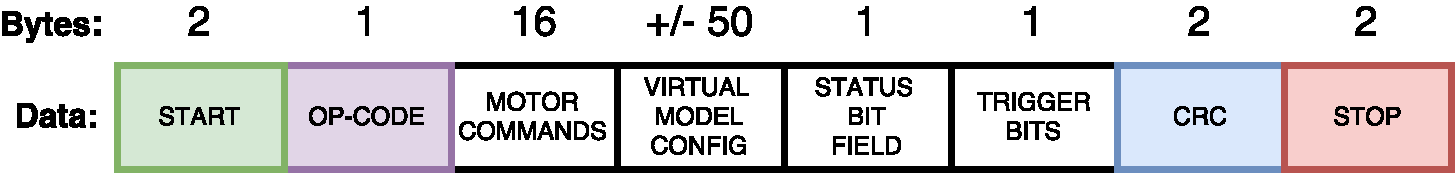
\includegraphics[clip, trim=0cm 0cm 0cm 0cm, page = 1, width=1\textwidth]{images/comms/pc-tx-packet.pdf} 
\caption{PC TX packet structure.}
\label{fig:pc-tx-packet}
\end{figure}

\begin{figure}
\centering
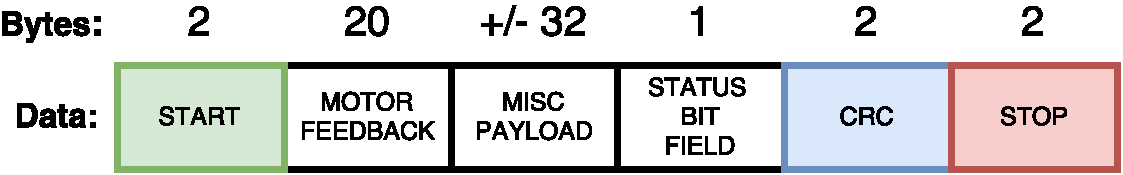
\includegraphics[clip, trim=0cm 0cm 0cm 0cm, page = 1, width=1\textwidth]{images/comms/pc-rx-packet.pdf} 
\caption{PC RX packet structure.}
\label{fig:pc-rx-packet}
\end{figure}


\subsection{Integrity Checking}
CRC ...

\subsection{Encoding and Decoding}
\subsubsection{PC Packet}
\subsubsection{Motor Driver Packet}
SeqBits bits 2-5 switch case


\section{Peripheral Configuration}

\begin{figure}
\centering
\includegraphics[clip, trim=1cm 7cm 1cm 7cm, page = 2, width=0.8\textwidth]{pdfs/BalekaSTMConfig.pdf} 
\caption{STM32F4 microcontroller peripheral configuration.}
\label{fig:microcontroller-peripheral-config}
\end{figure}

\subsection{Protocol}
\subsection{Data Rates}
\subsection{Direct Memory Access}


\begin{figure}
\centering
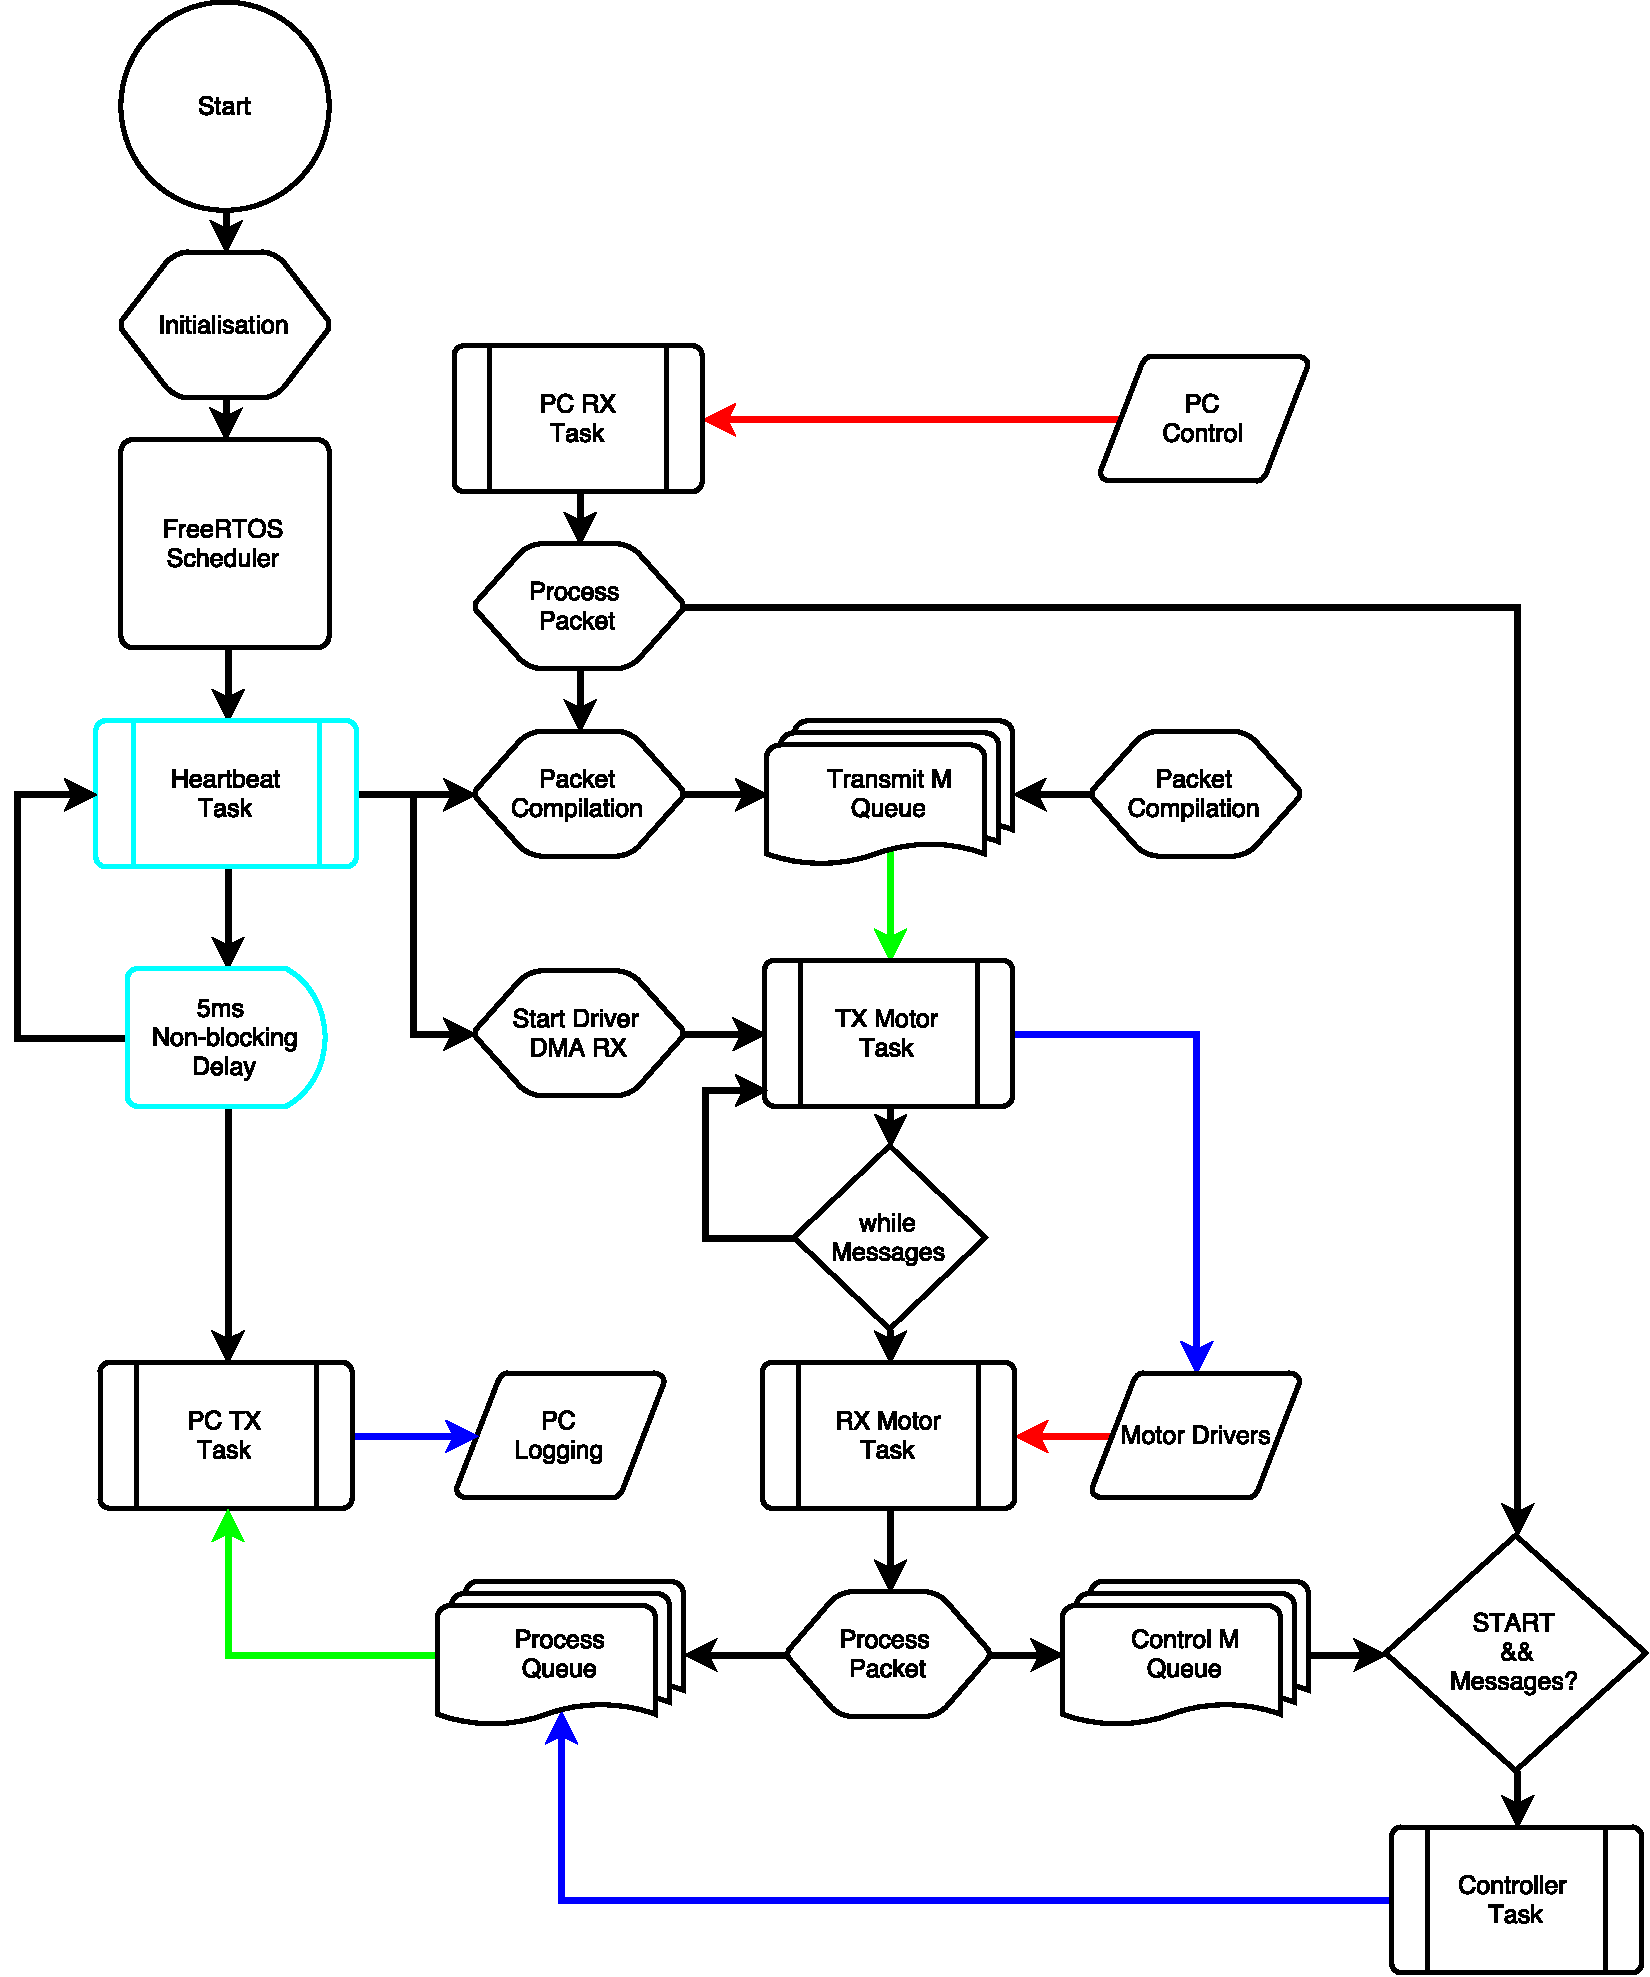
\includegraphics[width=1\textwidth]{images/comms/communication-flow-diagram.pdf} 
\caption{FreeRTOS communication protocol flow diagram.}
\label{fig:FreeRTOS communication protocol flow diagram.}
\end{figure}

\begin{figure}
\centering
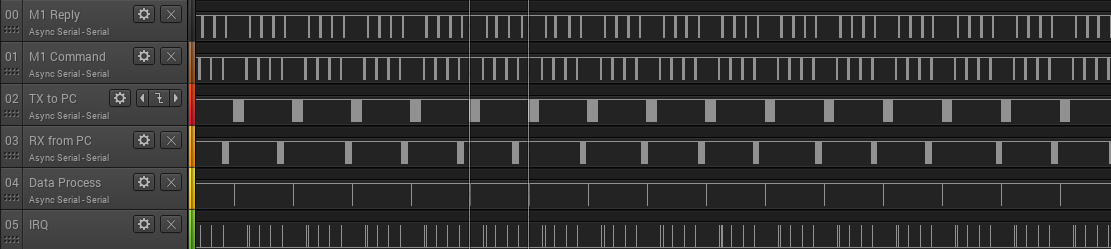
\includegraphics[width=1\textwidth]{images/comms/pc-packet-timing-data} 
\caption{Communication protocol packet timing with 5 ms sampling rate.}
\label{fig:packet-timing}
\end{figure}

\begin{table}
\centering
\begin{tabular}{llllll}
\textbf{Command}       & \textbf{Index} & \textbf{Op-Code} & \textbf{TX CB} & \textbf{TX CRC1} & \textbf{RX  CB} \\
\textbf{Kill Bridge}   & 1              & 0001             & 0x06           & 0xCBB6           & 0x04            \\
\textbf{Write Enable}  & 2              & 0010             & 0x0A           & 0x3624           & 0x08            \\
\textbf{Bridge Enable} & 3              & 0100             & 0x12           & 0x1AE0           & 0x10            \\
\textbf{Set Current}   & 4              & 0011             & 0x0E           & 0xBF7B           & 0x0C            \\
\textbf{Read Current}  & 5              & 1100             & 0x31           & 0x9772           & 0x32            \\
\textbf{Read Position} & 6              & 1111             & 0x3D           & 0xD310           & 0x3E            \\
\textbf{Read Velocity} & 7              & 0101             & 0x15           & 0x5EAF           & 0x16            \\
\textbf{Set Position}  & 8              & 1010             & 0x2A           & 0x42C4           & 0x28           
\end{tabular}
\caption{Motor driver command protocol.}
\label{tab:motor-driver-protocol}
\end{table}

\section{Graphic User Interface}
\label{chap:Graphic User Interface}

To enable rapid prototyping, a basic pre-existing serial logging platform was used and plug-ins were developed to adapt the software for controlling, configuring, logging and live plotting of the Baleka robotic leg platform. 

qSerialTerm, described as "A Qt based Serial Port terminal emulator", was built upon. It is distributed under the GNU General Public License (GPL) v3, which allows distribution, customisation and even sale of software published under the license, so long as basic conditions are met. It is copyright 2012 by Jorge Aparicio who's software repository can be found on GitHub: \url{https://github.com/JorgeAparicio/qSerialTerm}.

Qt Creator CPP was used for the software development and can be compiled to run on both Linux and Windows platforms - for reference all development was completed on a Linux platform.

Three .cpp files were used for the majority of the added functionality, namely: CRC.c, framewidget.cpp and serialportwidget.cpp along with their respective header files and Qt forms.

\subsection{Serial Communication}

\begin{figure}
\centering
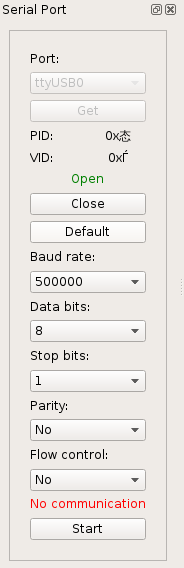
\includegraphics[width=0.3\textwidth]{images/gui/serial-port}
\end{figure}

\subsection{Logging}

\begin{figure}
\centering
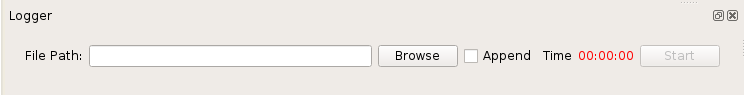
\includegraphics[width=0.8\textwidth]{images/gui/logger}
\end{figure}

\subsection{Live Plotting}

\begin{figure}
\centering
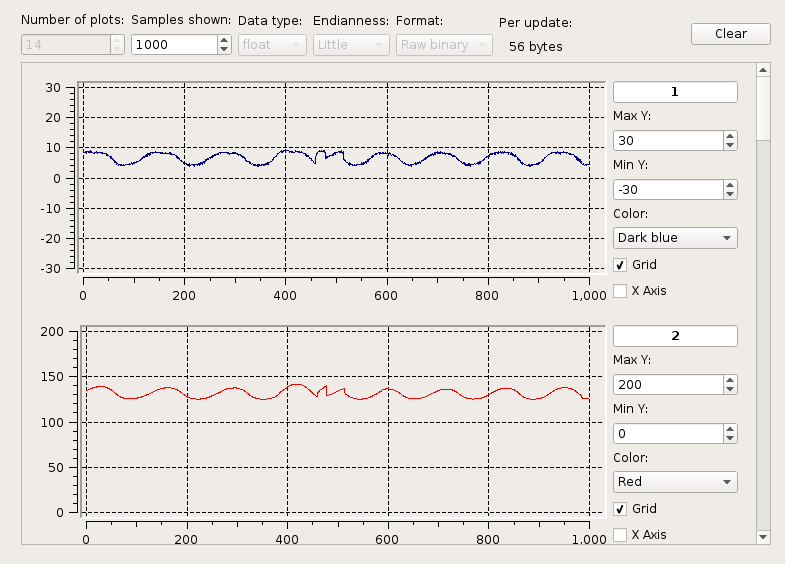
\includegraphics[width=0.7\textwidth]{images/gui/plotting}
\end{figure}

\subsection{Control Plug-in}

\begin{figure}
\centering
\subfloat[][Configuration \& On-board Control]{
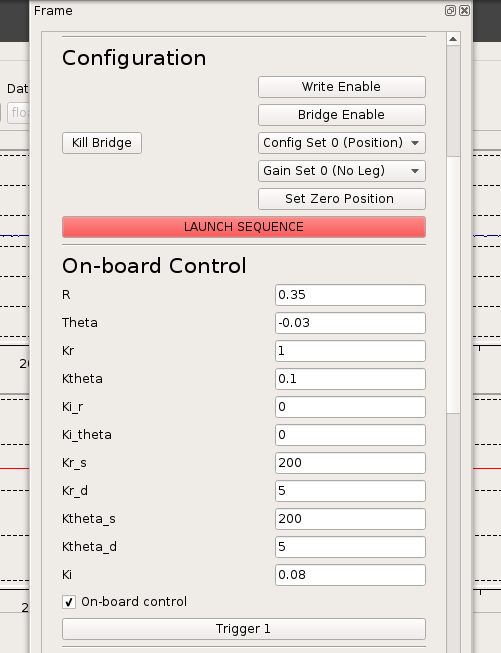
\includegraphics[width=0.4\textwidth]{images/gui/frame-1}
}
~
\subfloat[][Current/Position Control \& Control Loop Gains]{
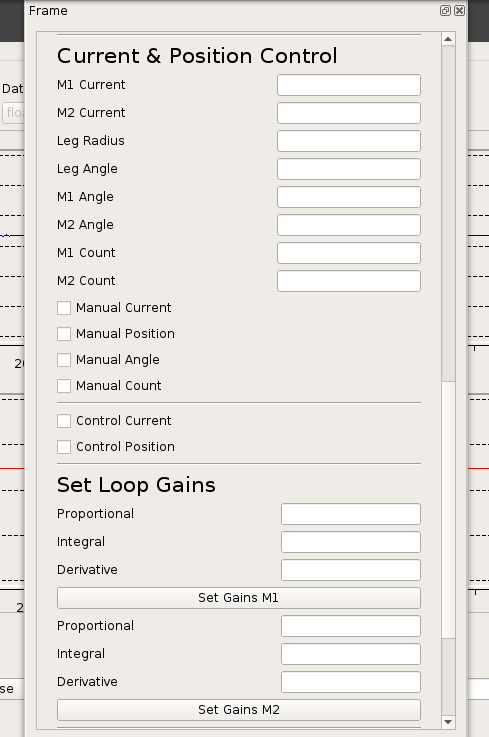
\includegraphics[width=0.4\textwidth]{images/gui/frame-2}
}
\caption{Control interface plug-in.}
\label{fig:Control interface plug-in} 
\end{figure}